%%% !TeX document-id = {7f856805-4d41-4d13-829b-b08b1a8ea49a}
 %%%  کلاس AUTthesis، نسخه اردیبهشت 1396
%%%   دانشگاه صنعتی امیرکبیر                 http://www.aut.ac.ir
%%%  تالار گفتگوی پارسی‌لاتک،       http://forum.parsilatex.com
%%%   آپدیت شده در آبان 95
%%      پشتیبانی و راهنمایی          badali_farhad@yahoo.com
%%%
%%%   بازبینی و اصلاح شده در اردیبهشت ماه 1396
%%%  Tested via TeXstudio in TeXlive 2014,‌‌ 2015 & 2016.
%%%

%-----------------------------------------------------------------------------------------------------
%        روش اجرا.: 2 بار F1 ، 2 بار  F11(به منظور تولید مراجع) ، دوبار Ctrl+Alt+I (به منظور تولید نمایه) و دو بار F1 -------> مشاهده Pdf
%%%%%%%%%%%%%%%%%%%%%%%%%%%%%%%%%%%%%%%%%%%%%%%%%%%%%%
%   TeXstudio as your IDE
%%  برای compile در TeXstudio تنها کافی است منوی Options->Configure TeXstudio را زده و در پنجره Configure TeXstudio در بخش Build گزینه Default Compiler را به XeLaTeX تغییر دهید. سند شما به راحتی compile خواهد شد.
%   F1 & F5 : Build & view
%   F6      : Compile
%   F7      : View
%   --------------
%   شما می‌توانید این نرم‌افزار را از سایت زیر دریافت کنید. برای استفاده از این نرم‌افزار باید پیش از نصب آن TeXlive را نصب کرده باشید.
%   TeXstudio.org
%   این سند با نسخه‌های 2014، 2015 و 2016 نرم‌افزار TeXlive در محیط TeXstudio آزمایش شده است.
%   نکته: در هنگام compile با نرم‌افزار TeXstudio فایل اصلی حتما باید باز باشد ولی نیازی نیست که روی tab آن باشید.
%	همچنین در پوشه LookAtMe فایلهای png برای راهنمایی وجود دارند.
%	برای ساخت میانبر نیم فاصله نیز به فایلهای پوشه LookAtMe را نگاه کنید.
%   باآرزوی پیروزی برای شما
%   آریا
%%%%%%%%%%%%%%%%%%%%%%%%%%%%%%%%%%%%%%%%%%%%%%%%%%%%%%
%        اگر قصد نوشتن رساله دکتری را دارید، در خط زیر به جای msc،
%      کلمه phd را قرار دهید. کلیه تنظیمات لازم، به طور خودکار، اعمال می‌شود.
%%% !TEX TS-program = XeLaTeX
\documentclass[oneside,msc]{AUTthesis}
%       فایل commands.tex را حتماً به دقت مطالعه کنید؛ چون دستورات مربوط به فراخوانی بسته زی‌پرشین 
%       و دیگر بسته‌ها و ... در این فایل قرار دارد و بهتر است که با نحوه استفاده از آنها آشنا شوید. توجه شود برای نسخه نهایی پایان‌نامه حتماً hyperref را 
%        غیرفعال کنید.


% در این فایل، دستورها و تنظیمات مورد نیاز، آورده شده است.
%-------------------------------------------------------------------------------------------------------------------
% در ورژن جدید زی‌پرشین برای تایپ متن‌های ریاضی، این سه بسته، حتماً باید فراخوانی شود.
\usepackage{amsthm,amssymb,amsmath,amsfonts}
% بسته‌ای برای تنطیم حاشیه‌های بالا، پایین، چپ و راست صفحه
\usepackage[top=30mm, bottom=30mm, left=25mm, right=30mm]{geometry}
% بسته‌‌ای برای ظاهر شدن شکل‌ها و تصاویر متن
\usepackage{graphicx}
\usepackage{color}
%بسته‌ای برای تنظیم فاصله عمودی خط‌های متن
\usepackage{setspace}
\setstretch{1.3}
\usepackage{tocstyle}
\usetocstyle{standard}
\usepackage{titleps}
\usepackage{titletoc}
\usepackage{tocloft}
\usepackage{multirow}
\usepackage{tabularx}
\usepackage{booktabs}
%با فعال کردن بسته زیر فوت‌نوت‌ها در هر صفحه ریست می‌شوند. حالت پیش‌فرض آن ریست شدن در هر فصل می‌باشد.
%\usepackage[perpage]{footmisc}
\usepackage{enumitem}
%\usepackage{titlesec}
% بسته‌ و دستوراتی برای ایجاد لینک‌های رنگی با امکان جهش
\usepackage[pagebackref=false,colorlinks,linkcolor=blue,citecolor=red]{hyperref}
\usepackage[nameinlink]{cleveref}%capitalize,,noabbrev
 \AtBeginDocument{%
    \crefname{equation}{برابری}{equations}%
    \crefname{chapter}{فصل}{chapters}%
    \crefname{section}{بخش}{sections}%
    \crefname{appendix}{پیوست}{appendices}%
    \crefname{enumi}{مورد}{items}%
    \crefname{footnote}{زیرنویس}{footnotes}%
    \crefname{figure}{شکل}{figures}%
    \crefname{table}{جدول}{tables}%
    \crefname{theorem}{قضیه}{theorems}%
    \crefname{lemma}{لم}{lemmas}%
    \crefname{corollary}{نتیجه}{corollaries}%
    \crefname{proposition}{گزاره}{propositions}%
    \crefname{definition}{تعریف}{definitions}%
    \crefname{result}{نتیجه}{results}%
    \crefname{example}{مثال}{examples}%
    \crefname{remark}{نکته}{remarks}%
    \crefname{note}{یادداشت}{notes}%
}
% چنانچه قصد پرینت گرفتن نوشته خود را دارید، خط بالا را غیرفعال و  از دستور زیر استفاده کنید چون در صورت استفاده از دستور زیر‌‌، 
% لینک‌ها به رنگ سیاه ظاهر خواهند شد که برای پرینت گرفتن، مناسب‌تر است
%\usepackage[pagebackref=false]{hyperref}
% بسته‌ لازم برای تنظیم سربرگ‌ها
\usepackage{fancyhdr}
% بسته‌ای برای ظاهر شدن «مراجع»  در فهرست مطالب
\usepackage[nottoc]{tocbibind}
% دستورات مربوط به ایجاد نمایه
\usepackage{makeidx,multicol}
\setlength{\columnsep}{1.5cm}
%\usepackage{tensor}
\usepackage[all]{xy}
\usepackage{tikz}
\usetikzlibrary{arrows}
%%%%%%%%%%%%%%%%%%%%%%%%%%
\usepackage{verbatim}
\makeindex
\usepackage{sectsty}
% فراخوانی بسته زی‌پرشین و تعریف قلم فارسی و انگلیسی
\usepackage{xepersian}%[extrafootnotefeatures]
\SepMark{-}
%حتماً از تک لایو 2014 استفاده کنید.
\settextfont[Scale=1.1,Path=fonts/]{BNazanin}
\setlatintextfont{Times New Roman}
\renewcommand{\labelitemi}{$\bullet$}
%%%%%%%%%%%%%%%%%%%%%%%%%%
% چنانچه می‌خواهید اعداد در فرمول‌ها، انگلیسی باشد، خط زیر را غیرفعال کنید.
%در غیر اینصورت حتماً فونت PGaramond را نصب کنید.
%\setdigitfont[Scale=1.1]{PGaramond}%%Yas
%%%%%%%%%%%%%%%%%%%%%%%%%%
% تعریف قلم‌های فارسی اضافی برای استفاده در بعضی از قسمت‌های متن
\defpersianfont\nastaliq[Scale=2,Path=fonts/]{IranNastaliq}
\defpersianfont\chapternumber[Scale=3,Path=fonts/]{BNazanin}
\chapterfont{\centering}%
%%%%%%%%%%%%%%%%%%%%%%%%%%
% دستوری برای تغییر نام کلمه «اثبات» به «برهان»
\renewcommand\proofname{\textbf{برهان}}

% دستوری برای تغییر نام کلمه «کتاب‌نامه» به «منابع و مراجع«
\renewcommand{\bibname}{منابع و مراجع}


% Headings for every page of ToC, LoF and Lot
\setlength{\cftbeforetoctitleskip}{-1.2em}
\setlength{\cftbeforelottitleskip}{-1.2em}
\setlength{\cftbeforeloftitleskip}{-1.2em}
\setlength{\cftaftertoctitleskip}{-1em}
\setlength{\cftafterlottitleskip}{-1em}
\setlength{\cftafterloftitleskip}{-1em}
%%\makeatletter
%%%%\renewcommand{\l@chapter}{\@dottedtocline{1}{1em\bfseries}{1em}}
%%%%\renewcommand{\l@section}{\@dottedtocline{2}{2em}{2em}}
%%%%\renewcommand{\l@subsection}{\@dottedtocline{3}{3em}{3em}}
%%%%\renewcommand{\l@subsubsection}{\@dottedtocline{4}{4em}{4em}}
%%%%\makeatother


\newcommand\tocheading{\par عنوان\hfill صفحه \par}
\newcommand\lofheading{\hspace*{.5cm}\figurename\hfill صفحه \par}
\newcommand\lotheading{\hspace*{.5cm}\tablename\hfill صفحه \par}

\renewcommand{\cftchapleader}{\cftdotfill{\cftdotsep}}
\renewcommand{\cfttoctitlefont}{\hspace*{\fill}\LARGE\bfseries}%\Large
\renewcommand{\cftaftertoctitle}{\hspace*{\fill}}
\renewcommand{\cftlottitlefont}{\hspace*{\fill}\LARGE\bfseries}%\Large
\renewcommand{\cftafterlottitle}{\hspace*{\fill}}
\renewcommand{\cftloftitlefont}{\hspace*{\fill}\LARGE\bfseries}
\renewcommand{\cftafterloftitle}{\hspace*{\fill}}

%%%%%%%%%%%%%%%%%%%%%%%%%%
% تعریف و نحوه ظاهر شدن عنوان قضیه‌ها، تعریف‌ها، مثال‌ها و ...
%برای شماره گذاری سه تایی قضیه ها
\theoremstyle{definition}
\newtheorem{definition}{تعریف}[section]
\newtheorem{remark}[definition]{نکته}
\newtheorem{note}[definition]{یادداشت}
\newtheorem{example}[definition]{نمونه}
\newtheorem{question}[definition]{سوال}
\newtheorem{remember}[definition]{یاداوری}
\theoremstyle{theorem}
\newtheorem{theorem}[definition]{قضیه}
\newtheorem{lemma}[definition]{لم}
\newtheorem{proposition}[definition]{گزاره}
\newtheorem{corollary}[definition]{نتیجه}
%%%%%%%%%%%%%%%%%%%%%%%%
%%%%%%%%%%%%%%%%%%%
%%% برای شماره گذاری چهارتایی قضیه ها و ...
%%\newtheorem{definition1}[subsubsection]{تعریف}
%%\newtheorem{theorem1}[subsubsection]{قضیه}
%%\newtheorem{lemma1}[subsubsection]{لم}
%%\newtheorem{proposition1}[subsubsection]{گزاره}
%%\newtheorem{corollary1}[subsubsection]{نتیجه}
%%\newtheorem{remark1}[subsubsection]{نکته}
%%\newtheorem{example1}[subsubsection]{مثال}
%%\newtheorem{question1}[subsubsection]{سوال}

%%%%%%%%%%%%%%%%%%%%%%%%%%%%

% دستورهایی برای سفارشی کردن صفحات اول فصل‌ها
\makeatletter
\newcommand\mycustomraggedright{%
 \if@RTL\raggedleft%
 \else\raggedright%
 \fi}
\def\@makechapterhead#1{%
\thispagestyle{style1}
\vspace*{20\p@}%
{\parindent \z@ \mycustomraggedright %\@mycustomfont
\ifnum \c@secnumdepth >\m@ne
\if@mainmatter

\bfseries{\Huge \@chapapp}\small\space {\chapternumber\thechapter}
\par\nobreak
\vskip 0\p@
\fi
\fi
\interlinepenalty\@M 
\Huge \bfseries #1\par\nobreak
\vskip 120\p@

}

%\thispagestyle{empty}
\newpage}
\bidi@patchcmd{\@makechapterhead}{\thechapter}{\tartibi{chapter}}{}{}
\bidi@patchcmd{\chaptermark}{\thechapter}{\tartibi{chapter}}{}{}
\makeatother

\pagestyle{fancy}
\renewcommand{\chaptermark}[1]{\markboth{\chaptername~\tartibi{chapter}: #1}{}}

\fancypagestyle{style1}{
\fancyhf{} 
\fancyfoot[c]{\thepage}
\fancyhead[R]{\leftmark}%
\renewcommand{\headrulewidth}{1.2pt}
}


\fancypagestyle{style2}{
\fancyhf{}
\fancyhead[R]{چکیده}
\fancyfoot[C]{\thepage{}}
\renewcommand{\headrulewidth}{1.2pt}
}

\fancypagestyle{style3}{%
  \fancyhf{}%
  \fancyhead[R]{فهرست نمادها}
  \fancyfoot[C]{\thepage}%
  \renewcommand{\headrulewidth}{1.2pt}%
}

\fancypagestyle{style4}{%
  \fancyhf{}%
  \fancyhead[R]{فهرست جداول}
  \fancyfoot[C]{\thepage}%
  \renewcommand{\headrulewidth}{1.2pt}%
}

\fancypagestyle{style5}{%
  \fancyhf{}%
  \fancyhead[R]{فهرست اشکال}
  \fancyfoot[C]{\thepage}%
  \renewcommand{\headrulewidth}{1.2pt}%
}

\fancypagestyle{style6}{%
  \fancyhf{}%
  \fancyhead[R]{فهرست مطالب}
  \fancyfoot[C]{\thepage}%
  \renewcommand{\headrulewidth}{1.2pt}%
}

\fancypagestyle{style7}{%
  \fancyhf{}%
  \fancyhead[R]{نمایه}
  \fancyfoot[C]{\thepage}%
  \renewcommand{\headrulewidth}{1.2pt}%
}

\fancypagestyle{style8}{%
  \fancyhf{}%
  \fancyhead[R]{منابع و مراجع}
  \fancyfoot[C]{\thepage}%
  \renewcommand{\headrulewidth}{1.2pt}%
}
\fancypagestyle{style9}{%
  \fancyhf{}%
  \fancyhead[R]{واژه‌نامه‌ی فارسی به انگلیسی}
  \fancyfoot[C]{\thepage}%
  \renewcommand{\headrulewidth}{1.2pt}%
}
%


%دستور حذف نام لیست تصاویر و لیست جداول از فهرست مطالب
\newcommand*{\BeginNoToc}{%
  \addtocontents{toc}{%
    \edef\protect\SavedTocDepth{\protect\the\protect\value{tocdepth}}%
  }%
  \addtocontents{toc}{%
    \protect\setcounter{tocdepth}{-10}%
  }%
}
\newcommand*{\EndNoToc}{%
  \addtocontents{toc}{%
    \protect\setcounter{tocdepth}{\protect\SavedTocDepth}%
  }%
}
\newcounter{savepage}
\renewcommand{\listfigurename}{فهرست اشکال}
\renewcommand{\listtablename}{فهرست جداول}
%\renewcommand\cftsecleader{\cftdotfill{\cftdotsep}}
%%%%%%%%%%%%%%%%%%%%%%%%%%%%%
%%%%%%%%%%%%%%%%%%%%%%%%%%%%

\begin{document}
\baselineskip=.75cm
%% -!TEX root = AUTthesis.tex
% در این فایل، عنوان پایان‌نامه، مشخصات خود، متن تقدیمی‌، ستایش، سپاس‌گزاری و چکیده پایان‌نامه را به فارسی، وارد کنید.
% توجه داشته باشید که جدول حاوی مشخصات پروژه/پایان‌نامه/رساله و همچنین، مشخصات داخل آن، به طور خودکار، درج می‌شود.
%%%%%%%%%%%%%%%%%%%%%%%%%%%%%%%%%%%%
% دانشکده، آموزشکده و یا پژوهشکده  خود را وارد کنید
\faculty{دانشکده مهندسی کامپیوتر و فناوری اطلاعات}
% گرایش و گروه آموزشی خود را وارد کنید
\department{گرایش شبکه‌های کامپیوتری}
% عنوان پایان‌نامه را وارد کنید
\fatitle{زنجیره‌سازی کارکردهای مجازی سرویس شبکه با لحاظ محدودیت منابع مدیریتی}
% نام استاد(ان) راهنما را وارد کنید
\firstsupervisor{دکتر بهادر بخشی}
%\secondsupervisor{استاد راهنمای دوم}
% نام استاد(دان) مشاور را وارد کنید. چنانچه استاد مشاور ندارید، دستور پایین را غیرفعال کنید.
% \firstadvisor{نام کامل استاد مشاور}
%\secondadvisor{استاد مشاور دوم}
% نام نویسنده را وارد کنید
\name{پرهام}
% نام خانوادگی نویسنده را وارد کنید
\surname{الوانی}
%%%%%%%%%%%%%%%%%%%%%%%%%%%%%%%%%%
\thesisdate{شهریور ۱۳۹۸}

% چکیده پایان‌نامه را وارد کنید
\fa-abstract{
    مساله‌ی مجازی سازی توابع شبکه سعی دارد توابع شبکه را به صورت مجازی در شبکه جایگذاری نمایند و در ادامه
    با برقراری ارتباط میان آن‌ها سرویس‌هایی را فراهم آورد.
    یکی از مسائل در این روش پذیرش سرویس‌ها و قرار دادن آن‌ها بر روی زیرساخت است
    که در کارهایی زیادی به آن پرداخته شده است ولی یکی از اجزا معماری مجازی سازی کارکردهای
    شبکه بخش مدیریتی است که می‌بایست در کنار سرویس‌ها بر روی زیرساخت مستقر شود.
    در این رساله ما قصد داریم جایگذاری سرویس‌ها با لحاظ منابع مدیریتی را
    مدل‌سازی و حل نماییم.
}


% کلمات کلیدی پایان‌نامه را وارد کنید
\keywords{مجازی سازی کارکردهای شبکه، زنجیره‌سازی کارکردهای مجازی سرویس شبکه،بهینه‌سازی، بهینه‌سازی خطی صحیح}



\AUTtitle
%%%%%%%%%%%%%%%%%%%%%%%%%%%%%%%%%%
\vspace*{7cm}
\thispagestyle{empty}
\begin{center}

\includegraphics[height=5cm,width=12cm]{images/in-the-name-of-god}
\end{center}
% تاییدیه دفاع
% \newpage
\thispagestyle{empty}
%\fontsize{18pt}{19pt}\selectfont

\section*{صفحه فرم ارزیابی و تصویب پایان نامه- فرم تأیید اعضاء كميته دفاع}

\fontsize{12pt}{14pt}\selectfont
\renewcommand{\baselinestretch}{1.5}
\vspace*{1cm}
   در این صفحه فرم دفاع یا تایید و تصویب پایان نامه موسوم به فرم کمیته دفاع- موجود در پرونده آموزشی- را قرار دهید.
\vspace*{1cm}


\subsection*{نکات مهم:}
 
\begin{itemize}
\item
	نگارش پایان نامه/رساله باید به
	{\color{red}
		زبان فارسی
	}
	و بر اساس آخرین نسخه دستورالعمل و راهنمای تدوین پایان نامه های دانشگاه صنعتی امیرکبیر باشد.(دستورالعمل و راهنمای حاضر)
\item رنگ جلد پایان نامه/رساله چاپي كارشناسي، كارشناسي ارشد و دكترا  بايد به ترتيب مشكي، طوسي و سفيد رنگ باشد.  
\item چاپ و صحافی پایان نامه/رساله بصورت
{\color{red}
	پشت و رو(دورو)
}
بلامانع است و انجام آن توصيه مي شود. 
\end{itemize}
%%%%%%%%%%%%%%%%%%%%%%%%%%%%%%%%%%%%%%%%%%%%%%%%%%%%%%%%%%%%%%%%%%%%%%%%%%%%%%%%%%%%%%%%%%%%%%%%%%
%%%%%%%%%%%%%%%%%%%%%%%%%%%%%%%%%%%%%%%%%%%%%%%%%%%%%%%%%%%%%%%%%%%%%%%%%%%%%%%%%%%%%%%%%%%%%%%%%%
\newpage
\thispagestyle{empty}
\begin{picture}(50,50)
  \put(10,0){
\includegraphics[scale=.06]{images/fa-logo}}
  \put(4.5,-13){\footnotesize{دانشگاه صنعتی امیرکبیر}}
  \put(10.5,-27){\footnotesize{(پلی‌تکنیک تهران)}}
  \put(170,30){\bf{به نام خدا}}
  \put(140,-5){\Large\bf{تعهدنامه اصالت اثر}}
  \put(300,0){تاریخ: \datethesis}
\end{picture}

\vspace*{2.5cm}

اينجانب {\bf{\fname\ \lname}} متعهد می‌شوم که مطالب مندرج در این پایان‌نامه حاصل کار پژوهشی اینجانب تحت نظارت و راهنمایی اساتید دانشگاه صنعتی امیرکبیر بوده و به دستاوردهای دیگران که در این پژوهش از آنها استفاده شده است مطابق مقررات و روال متعارف ارجاع و در فهرست منابع و مآخذ ذکر گردیده است. این پایان‌نامه قبلاً برای احراز هیچ مدرک هم‌سطح یا بالاتر ارائه نگردیده است.

در صورت اثبات تخلف در هر زمان، مدرک تحصیلی صادر شده توسط دانشگاه از درجه اعتبار ساقط بوده و دانشگاه حق پیگیری قانونی خواهد داشت.


کلیه نتایج و حقوق حاصل از این پایان‌نامه متعلق به دانشگاه صنعتی امیرکبیر می‌باشد. هرگونه استفاده از نتایج علمی و عملی، واگذاری اطلاعات به دیگران یا چاپ و تکثیر، نسخه‌برداری، ترجمه و اقتباس از این پایان نامه بدون موافقت کتبی دانشگاه صنعتی امیرکبیر ممنوع است. 
نقل مطالب با ذکر مآخذ بلامانع است.\\
\vspace{2.5cm}


{\centerline {\bf{\fname\ \lname}}}
\vspace*{.2cm}
{\centerline{امضا}}
%%%%%%%%%%%%%%%%%%%%%%%%%%%%%%%%%
% چنانچه مایل به چاپ صفحات «تقدیم»، «نیایش» و «سپاس‌گزاری» در خروجی نیستید، خط‌های زیر را با گذاشتن ٪  در ابتدای آنها غیرفعال کنید.
% پایان‌نامه خود را تقدیم کنید
% نیایش خود را در فایل زیر بنویسید.
% \begin{acknowledgementpage}

\vspace{1.5cm}

{\nastaliq
{
 نويسنده پايان‌نامه، درصورت تمايل ميتواند برای سپاسگزاری پايان‌نامه خود را به شخص يا اشخاص و يا ارگان خاصی تقدیم نماید.
}}\end{acknowledgementpage}
\newpage
%سپاسگزاری را در فایل زیر بنویسید.
% %%%%%%%%%%%%%%%%%%%%%%%%%%%%%%%%%%%%
\newpage\thispagestyle{empty}
% سپاس‌گزاری
{\nastaliq
سپاس‌گزاری
}
\\[2cm]
در اینجا لازم می‌دانم از راهنمایی‌ها و مساعدت‌های اساتید عزیز و گرانقدرم
جناب آقای دکتر بخشی صمیمانه قدردانی و سپاس‌گزاری نمایم.
در ادامه از دوست خوبم بهروز فرکیانی که همواره من را راهنمایی کرده‌
و
از پدر و مادرم که همواره من را حمایت کرده‌اند تشکر می‌کنم.


در نهایت جا دارد از دوست، همکار و مدیر خوبم سینا سعیدی مدیریت فنی تیم منابع مشترک شرکت ایده گزین ارتباطات روماک تشکر کنم که بدون حمایت‌های ایشان نگارش این پایان نامه ممکن نبود.








% با استفاده از دستور زیر، امضای شما، به طور خودکار، درج می‌شود.
\signature








%%%%%%%%%%%%%%%%%%%%%%%%%%%%%%%%%%%%%%%%%
%%%%%%%%%%%%%%%%%%%%%%%%%%%%%%%%%کدهای زیر را تغییر ندهید.
\newpage\clearpage

\pagestyle{style2}

\vspace*{-1cm}
\section*{\centering چکیده}
%\addcontentsline{toc}{chapter}{چکیده}
\vspace*{.5cm}
\ffa-abstract
\vspace*{2cm}


{\noindent\large\textbf{واژه‌های کلیدی:}}\par
\vspace*{.5cm}
\fkeywords
%دستور زیر برای شماره گذاری صفحات قبل از فصل اول با حروف ابجد است.
\pagenumbering{alph}
%-----------------------------------------------------------------------------
%در فایل زیر دستورات مربوط به نمایش صفحات فهرست مطالب- فهرست اشکال و جداول است.
%{\pagestyle{style2}
%\tableofcontents}\newpage
%
%\listoffigures
\cleardoublepage
\pagestyle{style6}
\tableofcontents
\pagestyle{style6}
\cleardoublepage
%اگر لیست تصاویر و لیست جداول ندارید ، کدهای زیر را با گذاشتن % در ابتدای آنها، غیرفعال کنید.
\BeginNoToc
\addtocontents{lof}{\lofheading}% add heading to the first page in LoF
\pagestyle{style5}
\listoffigures
\thispagestyle{style5}
\cleardoublepage
\addtocontents{lot}{\lotheading}% add heading to the first page in LoT
\thispagestyle{style4}
\listoftables
\thispagestyle{style4}
%\cleardoublepage
%
\cleardoublepage
\setcounter{savepage}{\arabic{page}}
\mainmatter
\addtocontents{toc}{\tocheading}% add heading to the first page in ToC, after frontmatter entries
\EndNoToc
% در صورت تمایل می‌توانید با فعال کردن دستور بالا، لیست تصاویر را به  پایان‌نامه خود اضافه کنید.
%-------------------------------------------------------------------------symbols(فهرست نمادها)
% وجود لیست نمادها الزامیست.(لطفاً نمادهای خود را جایگذین نمادهای پیش‌فرض کنید.)
% %%%%%%%%%%%%%

{\centering\LARGE\textbf{فهرست نمادها}\par}%

\pagenumbering{alph}
\setcounter{page}{\thesavepage}
%\setcounter{page}{6}
\vspace*{1cm}

\pagestyle{style3}
%\thispagestyle{empty}
%\addcontentsline{toc}{chapter}{فهرست نمادها}
\symb{\text{ نماد}}{مفهوم}
\\
%مقادیر بالا را تغییر ندهید
%%%%%%%%%%%%%%%%%%%%%%%%%%%%%%%%%%%%%%%%%%%%%%%%%%%%%%%%%
\symb{V^{SFC}_{i, F}}{
    \small
    مجموعه گره‌های گراف زنجیره‌ی \(i\)ام
}
\symb{E^{SFC}_i}{
    \small
    مجموعه یال‌های گراف زنجیره‌ی \(i\)ام
}
\symb{V_S^{PN}}{
    \small
    مجموعه گره‌های گراف زیرساخت
}
\symb{E_S^{PN}}{
    \small
    مجموعه یال‌های گراف زیرساخت
}
\symb{x_h}{
    \small
    متغیر باینری که نشان می‌دهد زنجیره‌ی \(h\)ام
    پذیرفته شده است یا خیر
}
\symb{y_{wk}}{
    \small
    تعداد نمونه‌هایی از نوع \(k\)
    که روی سرور فیزیکی \(w\) فعال شده‌اند
}
\symb{z^k_{vw}}{
    \small
    متغیر باینری که نشان می‌دهد نمونه‌ی \(v\)
    از نوع \(k\)
    روی سرور فیزیکی \(w\)
    جایگذاری شده است یا خیر
}
\symb{\bar{y}_w}{
    \small
    تعداد نمونه‌هایی از \lr{VNFM} که روی سرور \(w\) فعال شده‌اند
}
\symb{\bar{z}_{hw}}{
    \footnotesize
    متغیر باینری که نشان می‌دهد زنجیره‌ی \(h\) توسط \lr{VNFM}ای که روی سرور \(w\) قرار گرفته است مدیریت می‌شود یا خیر
}
\symb{\tau^{(u,v)}_{ij}}{
    \scriptsize
    متغیر باینری که نشان می‌دهد یال مجازی بین نمونه‌های \(u\) و \(v\) برای نگاشت از یال فیزیکی بین گره‌های \(i\) و \(j\)
    استفاده می‌کند یا خیر
}
\symb{\bar{\tau}^{v}_{ij}}{
    \scriptsize
    متغیر باینری که نشان می‌دهد برای نگاشت ارتباط مدیریتی نمونه‌ی \(v\) از یال فیزیکی بین گره‌های \(i\) و \(j\)
    استفاده شده است یا خیر
}

%%%%%%%%%%%%%%%%%%%%%%%%%%%%%%%%%%%%%%%

\thispagestyle{style3}
\newpage
%\pagestyle{style1}
%%%%%%%%%%%%%%%%%%%%%%%%%%%%%%%%%%%%


\thispagestyle{empty}

\vspace*{1cm}

\newpage
\pagestyle{style1}
\pagenumbering{arabic}
%--------------------------------------------------------------------------chapters(فصل ها)
%\chapter{مقدمه}


بیشتر سرویس‌های شبکه بر روی سخت افزارهای اختصاصی به نام
\lr{middle box}
ساخته می‌شوند.
تنوع و تعداد رو به افزایش سرویس‌های جدیدی که توسط کاربران تقاضا می‌گردد
باعث هزینه‌های زیاد برای خرید و نگهداری
\lr{middle box}‌ها
توسط اپراتورها شده است.
به تازگی فراهم آورندگان شبکه
شروع به حرکت به سوی مجازی‌سازی و نرم‌افزاری کردن بسترهای شکبه کرده‌اند،
به این ترتیب آن‌ها قادر خواهند بود
سرویس‌های نوآورانه‌ای به کاربران ارائه بدهند.

مجازی‌سازی توابع شبکه‌ راهکاری است که برای همین منظور پیشنهاد شده است.
مجازی‌سازی توابع شبکه‌ در واقع راه‌حل‌های مشخصی را برای چالش‌های جای‌گذاری،
زنجیره‌سازی و هماهنگی سرویس‌های شبکه فراهم می‌آورد.

ایده‌ی اصلی مجازی‌سازی توابع شبکه جداسازی تجهیزات فیزیکی شبکه از کارکردهایی می‌باشد که
بر روی آن‌ها اجرا می‌شوند.
به این معنی که یک کاکرد شبکه مانند دیوار آتش می‌تواند بر روی یک
\lr{TSP}
به عنوان یک نرم‌افزار ساده فرستاده شود.
با این روش یک سرویس می‌تواند به مجموعه‌ای از کارکردهای مجازی شبکه‌ای که می‌توانند به صورت نرم‌افزاری پیاده‌سازی شده
و روی یک یا تعداد سرور استاندارد فیزیکی اجرا شوند، شکسته شود.
کارکرهای مجازی شبکه‌ای می‌توانند در مکان‌های مختلف بازمکان‌یابی یا نمونه‌سازی شوند بدون آنکه
نیاز به خریداری و نصب تجهیز جدیدی باشد.
\cite{Mijumbi2016}

\section{معماری \lr{NFV}}
با توجه به استاندارد \lr{ETSI} معماری \lr{NFV}
از سه عنصر کلیدی تشکیل شده است.
%\chapter{مفاهیم پایه}

\section{مقدمه}

راه اندازی و استقرار سرویس در صنعت مخابرات به طور سنتی بر این اساس است که اپراتورهای شبکه سخت‌افزارهای اختصاصی فیزیکی و تجهیزات لازم برای هر کارکرد در سرویس را در زیرساخت خود مستقر کنند.
فراهم کردن نیازمندی‌هایی مانند پایداری و کیفیت بالا منجر به اتکای فراهم کنندگان سرویس بر سخت‌افزارهای اختصاصی می‌شود. 
این درحالی است که نیازمندی کاربران به سرویس‌های متنوع و عموما با عمرکوتاه و نرخ بالای ترافیک افزایش یافته است.
بنابراین فراهم کنندگان سرویس‌ها باید مرتبا و به صورت پیوسته تجهیزات فیزیکی جدید را خریده، انبارداری کرده و مستقر کنند.
تمام این عملیات باعث افزایش هزینه های فراهم کنندگان سرویس می‌شود.
با افزایش تجهیزات، پیدا کردن فضای فیزیکی برای استقرار تجهیزات جدید به مرور دشوارتر می‌شود.
علاوه بر این باید افزایش هزینه و تاخیر ناشی از آموزش کارکنان برای کار با تجهیزات جدید را نیز در نظر گرفت.
بدتر این که هر چه نوآوری سرویس‌ها و فناوری شتاب بیشتری می‍گیرد، چرخه عمر سخت‌افزارها کوتاه‍تر می‍شود که مانع از ایجاد نوآوری در سرویس‌های شبکه می‌شود.

در روش سنتی استقرار سرویس شبکه، ترافیک کاربر باید از تعدادی کارکرد شبکه به ترتیب معینی عبور کند تا یک مسیر پردازش ترافیک ایجاد شود.
در حال حاضر این کارکردها به صورت سخت‌افزاری به یکدیگر متصل هستند و ترافیک با استفاده از جداول مسیریابی به سمت آن‌ها هدایت می‌شود.
چالش اصلی این روش در این است که استقرار و تغییر ترتیب کارکردها دشوار است.
به عنوان مثال، به مرور زمان با تغییر شرایط شبکه نیازمند تغییر همبندی و یا مکان کارکردها برای سرویس‌دهی بهتر به کاربران هستیم که نیاز به جا به جایی کارکردها و تغییر جداول مسیریابی دارد.
در روش سنتی این کار سخت و هزینه‌بر است که ممکن است خطاهای بسیاری در آن رخ دهد.
از جنبه دیگر، تغییر سریع سرویس‌های مورد نظر کاربران نیازمند تغییر سریع در ترتیب کارکردها است که در روش فعلی این تغییرات به سختی صورت گیرد.
بنابراین اپراتورهای شبکه نیاز به شبکه های قابل برنامه ریزی و ایجاد زنجیره سرویس کارکردها به صورت پویا پیدا کرده اند.

دو فناوری برای پاسخگویی به این چالش‌ها مطرح شد:

\begin{itemize}
    \item مجازی‌سازی کارکرد شبکه یا \lr{NFV}
    \item زنجیره‌سازی کارکردهای سرویس یا \lr{SFC}
\end{itemize}

با استفاده از مجازی‌سازی کارکردهای شبکه و اجرای آن‌ها بر روی سرورهای استاندارد با توان بالا،
امکان اجرای کارکردها بر روی سخت افزارهای عمومی را فراهم کرده است تا نیاز به تجهیزات سخت افزاری خاص منظوره کاهش یابد.
از طرف دیگر \lr{SFC} امکان تعریف زنجیره کارکردها را ارائه می‌کند که ایجاد
و انتخاب مسیرهای متفاوت برای پردازش ترافیک به صورت پویا و بدون ایجاد تغییر در زیرساخت فیزیکی را امکان‌پذیر می‌کند
با توجه به این فناوری‌ها، مسائل تحقیقاتی جدیدی مطرح شدند که از مهم‌ترین آن‌ها می‌توان تخصیص منابع بهینه به سرویس درخواستی کاربر را نام برد.

از آنجایی که از مفاهیم این فناور‌ی‌ها برای طراحی و تعریف مساله در این رساله استفاده شده است، نیازمند آشنایی با مفاهیم ابتدایی و اصول اولیه آن‌ها خواهیم بود.

بنابراین در این فصل به صورت خلاصه اجزای این فناوری‌ها را مرور خواهیم کرد و کاربردها، چالش‌ها و مسائل تحقیقاتی که در هر یک از این معماری‌ها وجود دارد را مورد بررسی قرار خواهیم داد.

\section{مجازی‌سازی کارکرد شبکه}

مجازی‌سازی کارکرد شبکه اصل جداسازی کارکرد شبکه به وسیله انتزاع سخت‌افزاری مجازی از سخت افزاری است که بر روی آن اجرا می‌شود.
هدف مجازی‌سازی کارکرد شبکه تغییر روش اپراتورهای شبکه در طراحی شبکه
با تکامل مجازی سازی استاندارد فناوری اطلاعات به منظور تجمیع تجهیزات شبکه
در سرورهای استاندارد، سوییچ‌ها و ذخیره‌سازها با توان بالا است.
یک سرور استاندارد با توان بالا سروری است که توسط اجزای استاندارد شده \lr{IT}،
مانند معماری \lr{x86}، ساخته شده و
در تعداد بالایی، مانند میلیون،
فروخته می‌شود.
ویژگی اصلی این سرورها این است که اجزای آن‌ها به راحتی از فروشندگان مختلف قابل خریداری و
تعویض است.
این تجهیزات می‌توانند در مراکز داده، گره‌های شبکه، یا مکان کاربران انتهایی قرار بگیرند.
این روند در
شکل
\ref{fig.6}
نیز توصیف شده است.

\begin{figure}[!h]
\center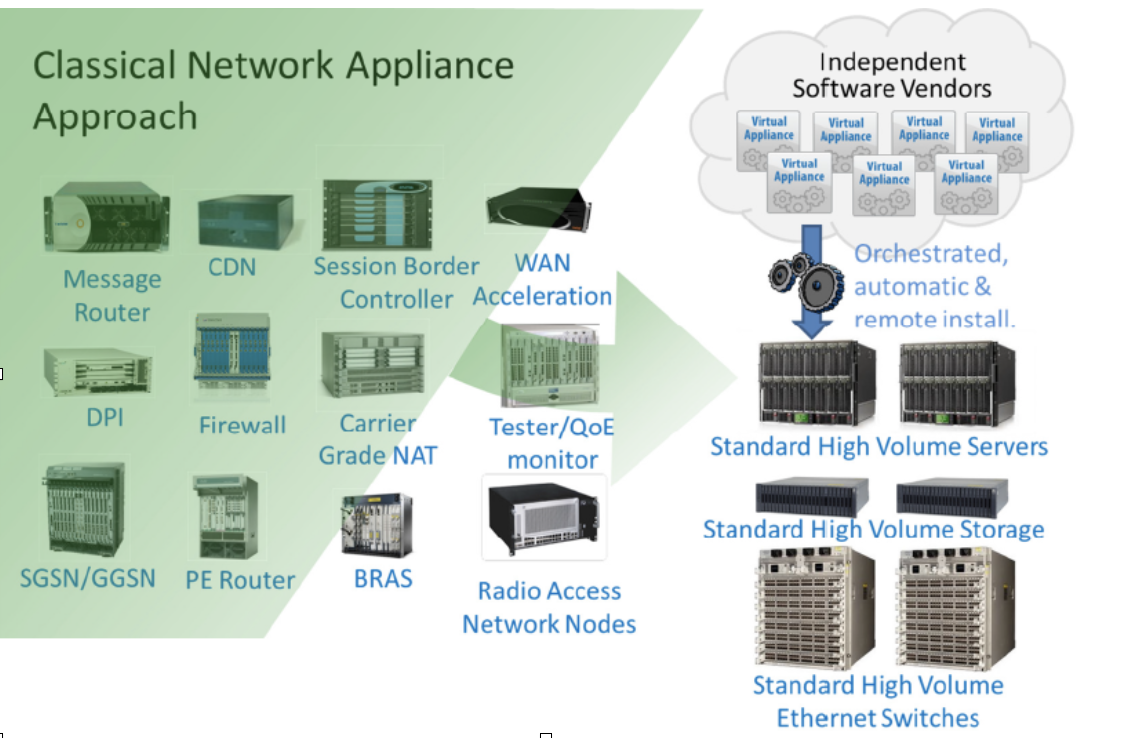
\includegraphics[scale=.5]{images/nfv-concept}
\caption{رویکرد \lr{NFV}}\label{fig.6}
\end{figure}

با استفاده از \lr{NFV}، انواع کارکردهای شبکه مانند دیواره آتش و \lr{NAT}
را می‌توان به صورت یک برنامه نرم‌افزاری از فروشندگان مختلف تهیه کرد و
آن‌ها را بر روی سرورهای با توان بالا اجرا کرد که نیاز به نصب تجهیزات خاص منظوره و
جدید را برطرف می‌سازد.

مزایا و اهداف اساسی که \lr{NFV} برای تحقق و دست‍یابی به آن‍ها شکل گرفته است عبارتند از:

\begin{itemize}
    \item
    کاهش هزینه‌های تجهیزات و مصرف انرژی از طریق تجمیع کارکردها بر روی سرورها و در نتیجه کاهش تعداد تجهیزات
    \item
    کاهش نیاز به آموزش کارکنان، افزایش دسترسی پذیری به سخت افزار و کاهش زمان بازیابی از خرابی سخت افزار به علت استفاده از سخت افزارهای استاندارد و عمومی
    \item
    افزایش سرعت عرضه محصول به بازار با کوتاه‌کردن چرخه نوآوری و تولید. در واقع \lr{NFV} به اپراتورهای شبکه کمک می‍کند تا چرخه بلوغ محصول را به اندازه قابل توجهی کاهش دهند.
    \item
    امکان‍پذیر بودن تعریف سرویس مورد نظر بر اساس نوع مشتری یا محل جغرافیایی. مقیاس سرویس‌ها می‍تواند به سرعت، بر اساس نیاز، گسترش یا کاهش یابد.
    \item
    تشویق به ایجاد نوآوری و ارائه سرویس‌های جدید و دریافت جریان‌های درآمدی تازه با سرعت بالا و ریسک پایین.
    \item
    افزایش توانایی  مقابله با خرابی کارکردها، قابلیت به اشتراک گذاری منابع بین کارکرد ها و پشتیابی از چند مشتری
\end{itemize}

سازمان‌های استانداردگذاری متعددی در استانداردسازی فناوری \lr{NFV} دخیل هستند که شاخص‌ترین آن‌ها موسسه استانداردهای مخابراتي اروپا (\lr{ETSI}) است.
در اواخر سال ۲۰۱۲،
\lr{ETSI NFV ISG}
توسط هفت اپراتور جهانی شبکه به منظور ارتقا ایده مجازی‌سازی کارکرد شبکه تأسیس شد.
\lr{NFV ISG}
تبدیل به یک بستر صنعتی اصلی برای توسعه چارچوب معماری \lr{NFV} و نیازمندی‌های آن شده است و اکنون بیش از ۲۵۰ سازمان با آن همکاری می‌کنند.
اسناد معماری \lr{NFV} به صورت عمومی و رایگان توسط \lr{ETSI NFV ISG} منتشر می‌شود.
ما در این رساله برای توصیف معماری \lr{NFV} از اسناد ارائه شده این سازمان استفاده می‌کنیم.

\section{معماری \lr{NFV}}

در این بخش مؤلفه‌های تشکیل‌دهنده معماری \lr{NFV} شرح داده می‍شوند.
هر یک از اجزای معماری می‍توانند توسط تولیدکنندگان متفاوتی تأمین شوند و به وسیله واسط‌هایی که توسط معماری \lr{NFV}
توصیف شده‌اند با یکدیگر در ارتباط باشند.
بنابراین معماری \lr{NFV} توصیف شده توسط \lr{ETSI} راه‌حلی با قابلیت مشارکت و هماهنگی چندین تولیدکننده مختلف را دارد.
با توجه به استاندارد \lr{ETSI} معماری \lr{NFV}
از سه عنصر کلیدی تشکیل شده است.
زیرساخت مجازی‌سازی کارکردهای شبکه،
کارکردهای مجازی شبکه‌ای و
\lr{NFV MANO}.
این اجزا در شکل \ref{fig.1} نمایش داده شده‌اند.

\begin{figure}[!h]
\center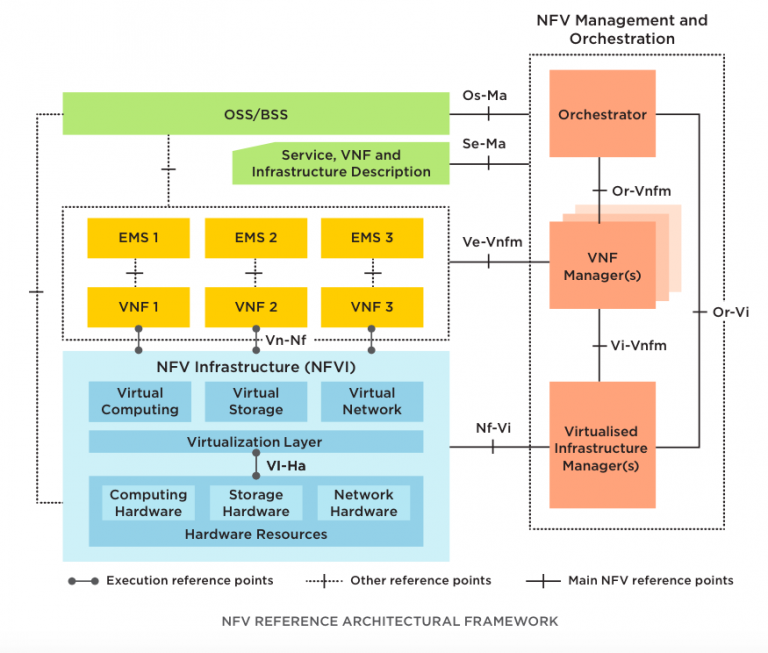
\includegraphics[scale=.5]{images/nfv-arch}
\caption{معماری مجازی‌سازی کارکردهای شبکه
}\label{fig.1}
\end{figure}

\begin{itemize}
    \item
    \lr{NFVI}: شامل منابع سخت افزاری و نرم‌افزاری لازم برای اجرای \lr{VNF}‌ها
    \item
    \lr{Service}: شامل \lr{VNF}‌ها که کارکردهای شبکه را پیاده‌سازی کرده‌اند، \lr{EMS} برای مدیریت \lr{VNF}‌ها و \lr{OSS/BSS} برای ارتباط با سیستم‌های مدیریت سنتی
    \item
    \lr{MANO}: که وظیفه مدیریت و هماهنگی سرویس‌ها و تخصیص منابع را برعهده دارد و از سه بخش \lr{NFVO}، \lr{VIM} و \lr{VNFM} تشکیل شده است.
\end{itemize}

\subsection{زیرساخت مجازی‌سازی کارکردهای شبکه یا \lr{NFVI}}
زیرساخت مجازی‌سازی کارکردهای شبکه ترکیبی از منابع نرم‌افزاری و سخت‌افزاری است
که محیطی برای نصب
کارکردهای مجازی شبکه فراهم می‌آورد.
منابع سخت‌افزاری شامل منابع محاسباتی،
ذخیره‌سازها و شبکه
(شامل لینک‌ها و گره‌ها)
هستند
که پردازش، ذخیره‌سازی و ارتباط را
برای کارکردهای مجازی شبکه فراهم می‌آورند.
منابع مجازی انتزاعی از منابع شبکه‌ای، پردازشی و ذخیر‌ه‌سازی هستند.
به وسیله انتزاع از طریق لایه‌ی مجازی‌سازی (بر پایه‌ی \lr{hypervisor})
منابع سخت افزاری در اختیار کارکردهای مجازی
قرار می‌گیرند که این منابع شامل منابع محاسباتی، شبکه‌ای و ذخیره‌سازی می‌باشند.

در مراکز داده‌ای ممکن است منابع پردازشی و ذخیره‌سازی تحت عنوان یک یا چند
ماشین مجازی نمایش داده شوند در حالی که شبکه‌های مجازی از لینک‌ها و گره‌های مجازی تشکیل می‌شوند.
شبکه‌های مجازی پیش از بحث مجازی‌سازی کارکردهای شبکه مدنظر بوده‌اند و روی آن‌ها کار شده است.
در واقع از شبکه‌های مجازی در مراکز داده‌ای جهت فراهم آوردن شبکه‌های مختلف و مجزا که به کاربران مختلفی تعلق دارند
استفاده شده است. راه‌حل‌های مختلفی برای پیاده‌سازی این شبکه‌ها وجود دارد. در بحث مجازی‌سازی کارکردهای شبکه‌، زیرساخت ارتباطی
مورد نیاز 
برای کارکردهای مجازی از طریق همین شبکه‌های مجازی فراهم آورده می‌شود.
یعنی مسائلی که پیشتر در بحث جایگذاری شبکه‌های مجازی مطرح بود
امروز جزئی از مسائل جایگذاری زنجیره‌های کارکرد سرویس می‌باشند.

\subsection{کارکردهای مجازی شبکه}
یک کارکرد شبکه، یک بلوک عملیاتی در زیرساخت شبکه است که عملکرد رفتاری و رابط‌های ارتباط با خارج خوش تعریف دارد.
مثال‌هایی از کارکردهای شبکه می‌تواند شامل
\lr{DHCP}
یا
\lr{firewall}
و ... باشد.
با این توضیحات کارکرد مجازی شبکه، پیاده‌سازی یک کارکرد شبکه است
که می‌تواند روی منابع مجازی شده اجرا شود.
از هر کارکرد شبکه می‌توان نمونه‌سازی کرده و چند نمونه را در شبکه مستقر ساخت. 
این نمونه‌ها می‌توانند برای سرویس‌دهی به زنجیره‌های مختلف استفاده شوند. از آنجایی که 
هر نمونه توان پردازشی محدودی دارد با افزایش تعداد نمونه‌ها می‌توان توان پردازشی یک کارکرد را نیز افزایش داد.

\subsection{\lr{EM}}
این مولفه کارکردهای \lr{FCAPS} را برای \lr{VNF} ها انجام می دهد که شامل مدیریت خطا، پیکربندی، امنیت، حسابداری و کارایی برای کارکردی است که \lr{VNF} ارائه می دهد. این مولفه ممکن است آگاه از مجازی کارکرد باشد و با همکاری \lr{VNFM} عملکردهای خودش را انجام بدهد.

\subsection{\lr{OSS/BSS}}
این مولفه، ترکیبی از سایر بخش های عملکردهای اپراتور است که در چارچوب معماری \lr{NFV} ارائه شده از طرف \lr{ETSI} قرار نمیگیرند. به عنوان مثال می تواند شامل مدیریت سیستم های \lr{Legacy} باشد.

\subsection{\lr{NFV MANO}}
بر اساس چهارچوب پیشنهادی \lr{ETSI}
وظیفه‌ی \lr{NFV MANO} فراهم آوردن کارکردهای لازم
برای تدارک و فرآیند‌های مشابه مانند تنظیم کردن و ... کارکردهای مجازی شبکه است.
\lr{NFV MANO} شامل هماهنگ کننده و مدیریت کننده چرخه‌ی زندگی
منابع سخت‌افزاری و نرم‌افزاری که مجازی‌سازی زیرساخت را پشتیبانی می‌کنند، است.
هر زنجیره نیاز دارد که حداقل توسط یک \lr{VNFM} مدیریت شود
تا مثلا خطاهای آن را تحت نظر قرار دهد و در صورت نیاز در قسمت دیگری از شبکه استقرار یابد.
مساله‌ی جایگذاری زنجیره‌ها بسیار مورد مطالعه قرار گرفته است، اما در این بین توجه لازم به نیاز این زنجیره‌ها به یک
\lr{VNFM}
صورت نپذیرفته است.

%\chapter{کارهای مرتبط}


در \cite{Eramo2016}
نویسندگان قصد دارند با در نظر گرفتن محدودیت ظرفیت لینک‌ها و محدودیت پردازشی نودها
بیشترین تعداد زنجیره‌ی کاکرد را بپذیرند. برای این کار یک مساله‌ی \lr{ILP}
طراحی می‌کنند و ثابت می‌کنند که این مساله \lr{NP-Hard} می‌باشد.
در این مقاله وجود \lr{VNFM} برای زنجیره‌ها در نظر گرفته نشده است.

در \cite{AbuLebdeh2017}
نویسندگان استفاده از \lr{VNFM} را مدنظر قرار داده‌اند
. در این مقاله فرض شده است که جایگذاری \lr{SFC}ها صورت گرفته است
و می‌خواهیم \lr{VNFM}ها را به گونه‌ای استقرار دهیم
که با رعایت شدن نیازمندی‌های کارآیی، هزینه‌ی عملیاتی سیستم حداقل شود.
مساله مطرح شده به صورت \lr{ILP} مدلسازی می‌شود.
این مقاله هزینه‌ی عملیاتی سیستم را تحت چهار عنوان دسته‌بندی می‌کند:
هزینه‌ی مدیریت چرخه‌ی زندگی، هزینه‌ی منابع محاسباتی، هزینه‌ی مهاجرت و هزینه‌ی بازنگاشت.
در این مقاله فرض می‌شود که هر نمونه از \lr{VNFM}ها می‌تواند به تعداد مشخصی از نمونه‌های \lr{VNF}
سرویس‌دهی کند و این سرویس‌دهی به نوع نمونه وابسته نیست.
این مقاله محدودیت‌های پردازشی و ظرفیتی را مدنظر قرار می‌دهد.

در \cite{Ghaznavi2017}
نویسندگان سه مرحله برای عملیات جایگذاری زنجیره‌های کارکرد سرویس معرفی می‌کنند:
انتخاب،
جابگذاری و
مسیریابی.
در این مقاله فرض می‌شود برای هر نوع \lr{VNF}
چند مدل مختلف با مصرف منابع مختلف وجود دارند که می‌توان از آن‌ها نمونه ساخت، در این مرحله مشخص می‌شود
از کدام مدل نمونه‌سازی صورت می‌گیرد.
این مقاله جایگذاری یک \lr{SFC} را مدل‌سازی می‌کند،
در این مقاله فرض می‌شود جریان ورودی و خروجی از هر نمونه برابر بوده و در واقع
\lr{VNF} تغییری بر روی ترافیک ایجاد نمی‌کند.
در مدل‌سازی این مقاله که به صورت \lr{ILP} می‌باشد هدف کاهش هزینه در جایگذاری \lr{SFC} داده شده می‌باشد.
با در نظر گرفتن مدل‌های مختلف برای \lr{VNF}ها در این مقاله
در صورتی که نیاز به پردازش ترافیک زیادی باشد، چند نمونه از یک نوع \lr{VNF}
ساخته می‌شود و ترافیک بین آن‌ها تقسیم می‌شود.

در \cite{Yu2017}
نویسندگان برای اولین‌بار مساله‌ی \lr{Traffic Streering}
با در نظر گرفتن \lr{QoS} و \lr{Reliability}
فرمول‌بندی کرده‌اند.
این مقاله کاربرد \lr{NFV} را در شبکه‌های موبایل مدنظر قرار داده است.
در این مقاله مساله به صورت \lr{Link-Path}
مدل‌سازی شده است و فرض شده است که مسیرهای ممکن برای جایگذاری کلاس‌های ترافیکی از پیش تعیین شده‌اند.
در این مقاله منظور از کیفیت سرویس تاخیر و گذردهی کلاس‌های ترافیکی می‌باشد و 
برای فراهم آوردن قابلیت اطمینان فرض می‌شود که خرابی‌ها به صورت دلخواه بوده و در صورت خرابی‌
بخشی از پهنای باند از دست می‌رود.


در \cite{Huang2017}
نویسندگان مساله‌ی جایگذاری و مسیریابی زنجیره‌های کارکرد سرویس را به صورت توامان مدل‌سازی می‌کنند،
در این مساله نویسندگان تاثیر دو پارامتر \lr{Coordination Effect} و \lr{Traffic-Change Effect}
را نیز مدنظر قرار داده‌اند.
زمانی که چند \lr{VM} در پیاده‌سازی یک کارکرد شبکه استفاده می‌شوند
نیاز است که بین این ماشین‌های مجازی هماهنگی صورت بگیرد.
برای این هماهنگی ارتباطاتی صورت می‌گیرد که دارای سربار بوده و به این سربار
\lr{Coordination Effect} می‌گویند.
هر کارکرد شبکه می‌تواند روی ترافیک ورودی خود تاثیر گذاشته و نرخ آن را تغییر دهد
که این موضوع را با \lr{Traffic-Change Effect} بیان می‌کنند.

در \cite{Chen2017}
نویسندگان قصد دارند به صورت قطعی کیفیت سرویس را گارانتی نمایند.
این مقاله پیاده‌سازی \lr{NFV} را با استفاده از \lr{SDN} هدف قرار می‌دهد
و برای محاسبه‌ی تاخیر، تاخیر پیام‌های کنترلی \lr{SDN} و
تاخیر جابجایی بسته‌ها را در نظر می‌گیرد.
برای پیشنهاد یک راه‌حل قطعی از \lr{Network Calculus}
استفاده می‌شود که شرایط مرزی را بررسی می‌کند.
این شرایط مرزی برای پیام‌های کنترلی محاسبه شده
و از آن تاخیر مورد نظر در جابجایی بسته‌ها بدست می‌آید
که با استفاده از آن یک مساله‌ی بهینه‌سازی با هدف رعایت تاخیر بدست آمده حاصل می‌شود.

در \cite{Ma2017}
نویسندگان پیاده‌سازی \lr{NFV} با \lr{SDN}
را هدف قرار داده‌اند و جایگذاری \lr{middle box}ها
با هدف توزیع‌بار را فرمول‌بندی کرده‌اند.
در واقع \lr{middle box}ها
در این مقاله به صورت مجازی بوده و همان کارکردهای مجازی شبکه می‌باشند.
مدل‌سازی صورت گرفته به صورت \lr{node link} صورت پذیرفته است.
هدف مساله مسیریابی چند مسیره برای تقاضا به صورتی است که در آن
\lr{link load ratio} برای تمام لینک‌ها می‌نیمم شود.
این مقاله تغییر ترافیک توسط کارکردها را نیز مدنظر قرار داده است.

در \cite{Jang2017}
مساله‌ی جایگذاری زنجیره‌های کاکرد سرویس با دو هدف کاهش مصرف انرژی و افزایش نرخ جریان پذیرفته شده
مدل‌سازی می‌شود. این مدل‌سازی با توجه به معماری \lr{IETF SFC} صورت پذیرفته است.
در مدلسازی این مقاله جزئیات زیادی مورد توجه قرار گرفته است که این امر باعث پیچیده شدن
فرمول‌بندی شده است.

در \cite{Eramo2017}
نویسندگان ابتدا مساله‌ی جایگذاری و مسیریابی \lr{VNF}ها را
در اوج ترافیک حل می‌کنند. در ادامه آن‌ها فرض می‌کنند که ترافیک به صورت دوره‌ای-ثابت می‌باشد
به این معنا که ترافیک در تعداد متناهی بازه‌ی زمانی تعریف شده و تکرار می‌شود.
با این فرض در ادامه مقاله مساله‌ی دیگری مبنی بر مهاجرت نمونه‌ها با توجه به تغییر ترافیک را مطرح می‌کند.
در این مهاجرت‌ها مقاله از توان مصرفی در مهاجرت صرف نظر کرده و تلاش می‌کند جریمه‌ای که بابت قطعی سرویس پرداخت می‌شود
و توان مصرفی کل سیستم را بهینه کند.

در \cite{Pham2017}
نویسندگان مساله‌ی توزیع‌بار در \lr{NFV} را بررسی می‌کنند،
آن‌ها در این مساله ویژگی‌های پایه‌ای \lr{NFV} در کنار استفاده از
روش \lr{ECMP} مدنظر قرار می‌دهد.
در روش \lr{ECMP} بار بین مبدا و مقصد
به صورت یکسان بین تمام مسیرها تقسیم می‌گردد.
در این مساله تعدادی تقاضا در نظر گرفته می‌شود که کوتاهترین مسیرها بین مبدا و مقصد آن‌ها مشخص است
و در نهایت بار در این مسیرها توزیع شده و کارکردها شبکه‌ای نیز در این مسیرها مستقر می‌شوند.

\begin{table}[h]
    \caption{مقایسه مقالات}
    \vspace{0.5cm}
    \begin{tabularx}{\textwidth}{|X|X|X|X|X|X|X|X|X|X|X|X|X|X|X|}
        \hline
        منبع &
        \multicolumn{4}{X|}{منابع تخصیص یافته} &
        \multicolumn{2}{X|}{محدودیت ظرفیت پردازشی نمونه} &
        \multicolumn{2}{X|}{برخط یا برون خط} &
        \multicolumn{2}{X|}{نگاشت کارکرد و لینک} &
        \multicolumn{2}{X|}{انتساب کارکرد} &
        \multicolumn{2}{X|}{اشتراک نمونه} \\
        \hline
        \lr{\#} &
        \lr{other} &
        \lr{MEM} &
        \lr{BW} &
        \lr{CPU} &
        دارد &
        ندارد &
        برخط &
        برون خط &
        کارکرد &
        لینک &
        یک نمونه &
        چند نمونه &
        دارد &
        ندارد \\
        \hline
    \end{tabularx}
\end{table}
%\chapter{تعریف مساله}

\section{مساله}
بیشینه کردن سود حاصل از پذیرفتن تقاضای زنجیره‌ کارکرد سرویس با در نظر گرفتن انتساب هر نمونه کارکرد مجازی شبکه به یک \lr{VNFM}.
همانطور که در مستند \cite{ETSI-MAN} نیز آمده است، نیاز است که هر یک نمونه‌های کارکردهای مجازی شبکه
توسط حداقل یک \lr{VNFM} مدیریت شوند.
در این مساله قصد داریم مساله پذیرش تقاضاهای زنجیره‌های کارکرد سرویس را با نظر گرفتن این نیازمندی در کنار
نیازمندی‌های پردازشی و پهنای‌باند هر یک از تقاضاها حل کنیم.
در ادامه به صورت خلاصه شرایط مساله را بررسی می‌کنیم:

\begin{itemize}
    \item توپولوژی زیرساخت شامل پهنای باند لینک‌ها و ظرفیت \lr{NFVI-PoP}ها\footnote{\lr{NFVI Point of Presence}} موجود است.
    \item \lr{n} تقاضای زنجیره‌ کارکرد سرویس به صورت کامل و از پیش مشخص شده داریم.
    \item هر تقاضا شامل نوع و تعداد نمونه‌های مجازی، پنهای باند لینک‌های مجازی و توپولوژی نمونه‌های مجازی می‌باشد.
    \item \lr{F} نوع کارکرد مجازی شبکه تعریف شده است که هر یک مقدار مشخصی از حافظه و توان پردازشی را مصرف می‌کنند.
    \item تعداد پردازنده‌هایی که به هر نمونه تخصیص می‌یابد با توجه به ترافیک ورودی نمونه مشخص می‌شود. این امر توسط اپراتور در زمان تعریف مساله ورودی صورت می‌گیرد.
    \item نمونه‌ها بین زنجیره‌ها به اشتراک گذاشته نمی‌شوند.
    \item محدودیت ظرفیت لینک‌ها
    \item محدودیت توان پردازش سرورهای فیزیکی با توجه به میزان حافظه و تعداد پردازنده‌ها
    \item برای مدیریت یکدست و آسان‌تر زنجیره‌ها و در عین حال جمع‌آوری راحت‌تر خطاها، برای هر زنجیره یک \lr{VNFM} فیزیکی تخصیص می‌دهیم.
    \item \lr{VNFM}ها می‌توانند بین زنجیره به اشتراک گذاشته شوند.
    \item هر نمونه از \lr{VNFM}ها می‌تواند تعداد مشخصی از نمونه‌های کارکرد مجازی شبکه را سرویس دهد. 
    \item برای ارتباط میان هر نمونه از \lr{VNFM}ها و \lr{VNF}ها پهنای باند مشخصی رزرو می‌گردد.
    \item در صورتی که \lr{NFVI-PoP} بتواند از \lr{VNFM} پشتیبانی نماید می‌توان به هر تعداد که ظرفیت آن اجازه می‌دهد بر روی آن \lr{VNFM} مستقر کرد.
    \item هر نمونه از \lr{VNFM} جهت استفاده نیاز به تهیه جواز\footnote{\lr{license}} دارد.
    \item توپولوژی می‌تواند دارای تعداد گره‌ی ورودی\footnote{\lr{ingress}} و خروجی\footnote{\lr{egress}} باشد.
    \item هر زنجیره می‌تواند دارای تعدادی نقطه‌ی ورودی و خروجی باشد که می‌بایست بر روی گره‌های ورودی و خروجی نگاشته شوند.
\end{itemize}

اگر جایگذاری \lr{VNFM}ها به صورت غیر برنامه‌ریزی شده صورت بپذیرد
ممکن است به تاخیرهای غیرقابل تحمل منجر شده و به این ترتیب تاثیر منفی بر روی کارآیی سیستم
داشته باشد.

یکی از وظایف \lr{VNFM}ها جمع‌آوری پیام‌های خطا می‌باشد،
برای این امر نیاز است که پهنای باند کوچک اما اختصاصی به \lr{VNFM}ها
تخصیص داده شود بنابراین نمی‌توان جایگذاری آن‌ها را با روش‌های سابق و مانند سایر
کارکردهای مجازی شبکه فرض کرد.

از آنجایی که \lr{VNFM}ها نیاز به مجوز دارند می‌توان با به اشتراک گذاشتن آن‌ها در هزینه‌های سیستم صرفه‌جویی کرد.

در نظرگرفتن \lr{VNFM} همراه با \lr{VNF}ها مساله‌ی جدیدی است.

\section{فرمول‌بندی}

هدف اصلی مساله پذیرش بیشترین تعداد تقاضا می‌باشد. در اینجا فرض می‌کنیم پذیرش هر تقاضا سودی منحصر به فرد خواهد داشت.
بنابراین تابع هدف به شکل زیر می‌باشد:

\begin{latin}\begin{align}
    max \sum_{h=1}^{T} c_hx_h - \sum_{w \in V_s^{PN}} licenseFee * \bar{y}_w
\end{align}\end{latin}

\begin{center}\begin{latin}\begin{tabular}{|c|p{10cm}|}
    \hline
    \(memory(k)\) & required RAM of VNF instance with type \(k\) in GB \\
    \hline
    \(core(k)\) & required CPU cores of VNF instance with type \(k\) \\
    \hline
    \(\hat{memory}\) & required RAM of VNFM in GB \\
    \hline
    \(\hat{core}\) & required CPU cores of VNFM \\
    \hline
    \(capacity\) & maximum number of VNF instances that VNFM can handle \\
    \hline
    \(len(h)\) & number of VNF instances in \(h\)th SFC request \\
    \hline
    \(type(v, k)\) & assuming the value 1 if the VNF instance \(v\) has type \(k\)  \\
    \hline
    \(bandwidth(u, v)\) & required bandwidth in link from VNF instance \(u\) to \(v\) \\
    \hline
    \(\hat{bandwidth}\) & required bandwidth in managmeent link \\
    \hline
    \(radius\) & maximum neighborhood distance for instance management \\
    \hline
    \(licenseFee\) & VNFM license fee that must pay for each VNFM \\
    \hline
    \(vnfSupport(w)\) & assuming the value 1 if the physical server \(w\) can support VNF instances \\
    \hline
    \(isManageable(k)\) & assuming the value 1 if the type \(k\) needs a manager \\
    \hline
    \(notManagableBy(w1, w2)\) & assuming the value 1 if the physical server \(w1\) cannot manage by physical server \(w2\) \\
    \hline
\end{tabular}\end{latin}\end{center}


\begin{center}\begin{latin}\begin{tabular}{|c|p{10cm}|}
    \hline
    \(x_h\) & binary variable assuming the value 1 if the \(h\)th SFC request is accepted; otherwise its value is zero \\
    \hline
    \(y_{wk}\) & the number of VNF instances of type \(k\) that are used in server \(w \in V_s^{PN}\) \\
    \hline
    \(z^k_{vw}\) & binary variable assuming the value 1 if the VNF node \(v \in \cup_{i=1}^{T} V_{i, F}^{SFC}\) is served by the VNF instance of type k in the server \(w \in V_s^{PN}\) \\
    \hline
    \(\bar{y}_w\) & the number of VNFMs (each vnfm has its capacity and license fee) that are used in server \(w \in V_s^{PN} \) \\
    \hline
    \(\bar{z}_{hw}\) & binary variable assuming the value 1 if \(h\)th SFC is assigned to VNFM on server \(w \in V_s^{PN}\) \\
    \hline
\end{tabular}\end{latin}\end{center}

برای هر نود اندازه‌ی مشخصی از حافظه \lr{RAM}
در نظر گرفته می‌شود که هر نمونه‌ی کارکرد با توجه به نوع آن مقدار مشخصی از این حافظه را مصرف می‌کند.
\lr{VNFM} نیز مقدار مشخصی از حافظه را مصرف می‌کند.

\begin{latin}
    \textit{Node Memory Constraint:}
    \begin{align}
        \sum_{k=1}^F y_{wk} memory(k) + \bar{y_w} \bar{memory} \le N_{ram}^{PN}(w)
        \quad
        \forall w \in V_s^{PN}
    \end{align}
\end{latin}

برای هر نود تعداد مشخصی از هسته‌های پردازنده در نظر گرفته می‌شود که هر نمونه‌ی کارکرد با توجه به نوع آن مقدار مشخصی از این تعداد را مصرف می‌کند.
\lr{VNFM} نیز مقدار مشخصی از تعداد هسته‌های پردازنده را مصرف می‌کند.

\begin{latin}
    \textit{Node CPU Constraint:}
    \begin{align}
        \sum_{k=1}^F y_{wk} core(k) + \bar{y_w} \bar{core} \le N_{core}^{PN}(w)
        \quad
        \forall w \in V_s^{PN}
    \end{align}
\end{latin}

اگر \lr{VNF}, \lr{v}
توسط \lr{VNF instance} نوع \lr{k}
روی سرور \lr{w} سرویس شود می‌بایست
\lr{VNF instance} نوع \lr{k}
روی سرور \lr{w} فعال شود.
توجه شود که
اشتراک گذاری \lr{VNF}ها پشتیبانی نمی‌گردد.

\begin{latin}
    \textit{Service Place Constraint:}
    \begin{align}
        \sum_{v \in \cup_{i=1}^T V_{i, F}^{SFC}} z_{vw}^k \le y_{wk}
        \quad
        \forall w \in V_s^{PN}, \forall k \in [1,\ldots, F]
    \end{align}
\end{latin}

اگر تقاضای \lr{h}ام پذیرفته شده باشد
می‌بایست تمام \lr{VNF node}های آن‌
سرویس شده باشند.
یک \lr{VNF} حداکثر یکبار سرویس داده شود.

\begin{latin}
    \textit{Service Constraint:}
    \begin{align}
        x_h = \sum_{k=1}^{F} \sum_{w \in V_{s}^{PN}} z_{vw}^{k}
        \quad
        \forall v \in V_{h,F}^{SFC}, \forall h \in [1,\ldots, T]
    \end{align}
\end{latin}

اگر تقاضای \lr{h}ام پذیرفته شده باشد
می‌بایست توسط یک \lr{VNFM} سرویس شده باشد.

\begin{latin}
    \textit{Manage Constraint:}
    \begin{align}
        x_h = \sum_{w \in V_{s}^{PN}} \bar{z}_{hw}
        \quad
        \forall h \in [1,\ldots, T]
    \end{align}
\end{latin}

محدودیت ظرفیت سرویس‌دهی \lr{VNFM}
این محدودیت براساس تعداد ماشین‌های محازی که هر
\lr{VNFM}
سرویس می‌دهد تعیین شده است.
در نظر داشته باشید که ممکن است برخی از انواع
\lr{VNF}‌ها
نیازی به مدیریت شدن نداشته باشند.

\begin{latin}
    \textit{Manage Capacity Constraint \& Manage Place Constraint:}
    \begin{align}
        \sum_{i=1}^{T} \bar{z}_{iw} * (len(i) - \sum_{v \in V_{i, F}^{SFC}} \sum_{k \in [1, \dots, F]} type(v, k) * isManageable(k)) \le capacity * \bar{y}_{w}
        \quad
        \forall w \in V_{s}^{PN}
    \end{align}
\end{latin}

اگر \lr{VNF}، \lr{v} توسط
\lr{instance}
نوع \lr{k} روی سرور \lr{w}
سرویس شود می‌بایست خود از نوع \lr{k} باشد.

\begin{latin}
    \textit{Type Constraint:}
    \begin{align}
        z_{vw}^{k} \le type(v, k)
        \quad
        \forall w \in V_{s}^{PN},
        \forall k \in [1,\ldots, F],
        \forall v \in \cup_{i=1}^T V_{i, F}^{SFC}
    \end{align}
\end{latin}

در صورتی که سرور \lr{w}
توانایی اجرای نمونه‌های \lr{VNF}
را نداشته باشد نباید نمونه‌ای روی آن قرار گیرد.

\begin{latin}
    \textit{VNF support constraint}
    \begin{align}
        \sum_{k \in [1, \dots, F]} y_{wk}  = M * vnfSupport(w)
        \quad
        w \in V_{s}^{PN}
    \end{align}
\end{latin}

برخی از سرورهای نمی‌توانند توسط سرورهای مشخصی مدیریت شوند.
این ویژگی به ادمین شبکه امکان مدیریت بیشتری می‌دهد و او می‌تواند با دست باز تمامی
سیاست‌های مورد نظرش را اعمال نماید.

\begin{latin}
    \textit{Manager to node support constraint}
    \begin{align}
        1 - z_{vw_1}^k + \bar{z}_{hw_2} = 0
        \quad
        & \forall w_1 \in V_s^{PN} \forall w_2 \in V_s^{PN} notManagableBy(w_1, w_2) = 1 \nonumber \\
        & \forall h \in [1,\dots,T],
        \forall v \in V_{h,F}^{SFC},
        \forall k \in [1,\dots,T]
    \end{align}
\end{latin}

\begin{center}\begin{latin}\begin{tabular}{|c|p{10cm}|}
    \hline
    \(\tau^{(u,v)}_{ij}\) & binary variable assuming the value 1 if the virual link \((u,v)\) is routed on the physical network link \((i,j)\) \\
    \hline
    \(\bar{\tau}^{v}_{ij}\) & binary variable assuming the value 1 if the managemnt of VNF node $v$ is routed on the physical network link \((i,j)\) \\
    \hline
\end{tabular}\end{latin}\end{center}

محدودیت زیر بقای جریان در لینک‌های مورد تقاضای کاربر را تضمین می‌کند.
\begin{latin}
    \textit{Flow Conservation:}
    \begin{align}
        \sum_{(i,j) \in E^{PN}} \tau_{ij}^{(u,v)} - \sum_{(j,i) \in E^{PN}} \tau_{ji}^{(u,v)} = \sum_{k=1}^{F} z_{ui}^{k} - \sum_{k=1}^{F} z_{vi}^{k} \nonumber \\
        \forall i \in V_{S}^{PN}, (u,v) \in E_{h}^{SFC}, h \in [1,\ldots, T]
    \end{align}
\end{latin}

محدودیت زیر بقای جریان در لینک‌های مدیریتی را تضمین می‌کند.
\begin{latin}
    \textit{Management flow Conservation:}
    \begin{align}
        \sum_{(i,j) \in E^{PN}} \bar{\tau}_{ij}^{v} - \sum_{(j,i) \in E^{PN}} \bar{\tau}_{ji}^{v} = \sum_{k=1}^{F} z_{vi}^{k} - \bar{z}_{hi} \nonumber \\
        \forall i \in V_{S}^{PN}, v \in V_{h, F}^{SFC}, h \in [1,\ldots, T]
    \end{align}
\end{latin}

محدودیت ظرفیت لینک‌ها
\begin{latin}
    \textit{Link Bandwidth Constraint:}
    \begin{align}
        \sum_{v \in \cup_{i=1}^{T} V_{i,F}^{SFC}} \bar{\tau}_{ij}^{v} * \bar{bandwidth} + \sum_{(u,v) \in \cup_{i=1}^{T} E_{i}^{SFC}} \tau_{ij}^{(u,v)} * bandwidth(u,v) \le C_{ij} \nonumber \\
        \forall (i, j) \in E^{PN}
    \end{align}
\end{latin}

شعاع همسایگی تضمین می‌کند که زمان سرویس‌دهی توسط
\lr{VNFM}ها
در یک بازه مشخص (از نظر تعداد هاب)
خواهد بود.
\begin{latin}
    \textit{Radius Constraint}
    \begin{align}
        \sum_{(i, j) \in E^{PN}} \bar{\tau}_{ij}^{v} \le radius
        \quad
        \forall v \in \cup_{i=1}^T V_{i, F}^{SFC}
    \end{align}
\end{latin}

%--------------------------------------------------------------------------appendix( مراجع و پیوست ها)
\chapterfont{\vspace*{-2em}\centering\LARGE}%

\appendix
\bibliographystyle{plain-fa}
\bibliography{references}
% \chapter*{‌پیوست}
\markboth{پیوست}{}
\addcontentsline{toc}{chapter}{پیوست}
موضوعات مرتبط با متن گزارش پایان نامه كه در يكی از گروه‌های زير قرار می‌گيرد، در بخش پيوست‌ها آورده شوند:
\begin{enumerate}
\item  اثبات های رياضی يا عمليات رياضی طولانی‌.‌
\item داده و اطلاعات نمونه (های) مورد مطالعه (\lr{Case Study}) چنانچه طولانی باشد‌.‌
\item نتايج كارهای ديگران چنانچه نياز به تفصيل باشد‌.‌
\item مجموعه تعاريف متغيرها و پارامترها، چنانچه طولانی بوده و در متن به انجام نرسيده باشد‌.‌
\end{enumerate}
% براي شماره‌گذاري روابط، جداول و اشكال موجود در پيوست‌ از ساختار متفاوتي نسبت به متن اصلي استفاده مي‌شود كه در زير به‌عنوان نمونه نمايش داده شده‌است. 
% \begin{equation}
%F=ma
%\end{equation}
\section*{کد میپل }
\begin{latin}
\begin{verbatim}

with(DifferentialGeometry):
with(Tensor):
DGsetup([x, y, z], M)
																	frame name: M
a := evalDG(D_x)
																	D_x
b := evalDG(-2 y z D_x+2 x D_y/z^3-D_z/z^2)


\end{verbatim}
\end{latin}
%--------------------------------------------------------------------------dictionary(واژه نامه ها)
%اگر مایل به داشتن صفحه واژه‌نامه نیستید، خط زیر را غیر فعال کنید.
\parindent=0pt
%%
\chapter*{واژه‌نامه‌ی فارسی به انگلیسی}
\pagestyle{style9}

\addcontentsline{toc}{chapter}{واژه‌نامه‌ی فارسی به انگلیسی}
%%%%%%
\begin{multicols*}{2}

{\bf آ}
%%\vspace*{3mm}

\vspace*{3mm}
{\bf ب}
%%\vspace*{3mm}

\vspace*{3mm}
{\bf پ}
%%\vspace*{3mm}

\vspace*{3mm}
{\bf ت}
%%\vspace*{3mm}

\vspace*{3mm}
{\bf ث}
%%\vspace*{3mm}

\vspace*{3mm}
{\bf ج}
%%\vspace*{3mm}

\vspace*{3mm}
{\bf چ}
%%\vspace*{3mm}

\vspace*{3mm}
{\bf ح}
%%\vspace*{3mm}

\vspace*{3mm}
{\bf خ}
%%\vspace*{3mm}

\vspace*{3mm}
{\bf د}
%%\vspace*{3mm}

\vspace*{3mm}
{\bf ر}
%%\vspace*{3mm}

\vspace*{3mm}
{\bf ز}
%%\vspace*{3mm}

\vspace*{3mm}
{\bf س}
%%\vspace*{3mm}

\vspace*{3mm}
{\bf ص}
%%\vspace*{3mm}

\vspace*{3mm}
{\bf ض}
%%\vspace*{3mm}

\vspace*{3mm}
{\bf ط}
%%\vspace*{3mm}

\vspace*{3mm}
{\bf ظ}
%%\vspace*{3mm}

\vspace*{3mm}
{\bf ع}
%%\vspace*{3mm}

\vspace*{3mm}
{\bf ف}
%%\vspace*{3mm}

\farsiTOenglish{فراهم‌آورنده‌ی شبکه}{Network Provider}



\vspace*{3mm}
{\bf ک}
%%\vspace*{3mm}

\vspace*{3mm}
{\bf گ}
%%\vspace*{3mm}

\vspace*{3mm}
{\bf م}
%%\vspace*{3mm}

\farsiTOenglish{مجازی‌سازی کارکردهای شبکه}{Network Function Virtualization}


\vspace*{3mm}
{\bf ن}
%%\vspace*{3mm}

\vspace*{3mm}
{\bf و}
%%\vspace*{3mm}

{\bf ه}
%%\vspace*{3mm}

{\bf ی}
%%\vspace*{3mm}


\end{multicols*}
% %%%%%%
\chapter*{واژه‌نامه}
\pagestyle{style9}
\lhead{\thepage}\rhead{واژه‌نامه}
\addcontentsline{toc}{chapter}{واژه‌نامه}

\englishTOfarsi{Interface}{رابط}

\englishTOfarsi{Application}{کاربرد}

\englishTOfarsi{Optimality Gap}{شکاف بهینه}

\englishTOfarsi{Edge}{یال}

\englishTOfarsi{Node}{گره}

\englishTOfarsi{Virtualization}{مجازی‌سازی}

\englishTOfarsi{Constraint}{محدودیت}

\englishTOfarsi{Heuristic}{مکاشفه‌ای}

\englishTOfarsi{Offline}{برون‌خط}

\englishTOfarsi{Online}{برخط}

\englishTOfarsi{Image}{تصویر}

\englishTOfarsi{Classifier}{دسته‌بند}

\englishTOfarsi{Forwarding}{جلورانی}

\englishTOfarsi{Function}{کارکرد}

\englishTOfarsi{Pod}{غلاف}

\englishTOfarsi{Aggregation}{تجمعی}

\englishTOfarsi{Edge}{لبه}

\englishTOfarsi{Instance}{نمونه}

\englishTOfarsi{Feasible Set}{مجموعه امکان‌پذیر}
%--------------------------------------------------------------------------index(نمایه)
%اگر مایل به داشتن صفحه نمایه نیستید، خط زیر را غیر فعال کنید.
\pagestyle{style7}
\printindex
\pagestyle{style7}
% %کلمات کلیدی انگلیسی
% \latinkeywords{NFV, SFC, Optimization, ILP}
%چکیده انگلیسی

\en-abstract{
In the old times, Network providers use hardware network functions to create their service chains, but a change in this manner is difficult and may cause many service distribution. SFC and NFV is the solution to this difficulty. By using SFC and NFV, providers can provision chains dynamically and then change them in runtime. One of the main requirements is management and monitoring for the chains.
In this research, we consider the chain acceptance problem subject to management resources. In the first step, we formulate
problem with ILP and then implement it in CPLEX framework. As we know, ILP problems are NP-Hard, so we need an NP solution to the problem. In this research, we create a heuristic algorithm and compare its result with the optimal solution. In the end, the heuristic solution produces near-optimal results in the polynomial time.
}
%%%%%%%%%%%%%%%%%%%%% کدهای زیر را تغییر ندهید.

\newpage
\thispagestyle{empty}
\begin{latin}
\section*{\LARGE\centering Abstract}

\een-abstract

\vspace*{.5cm}
{\large\textbf{Key Words:}}\par
\vspace*{.5cm}
\elatinkeywords
\end{latin}

%% در این فایل، عنوان پایان‌نامه، مشخصات خود و چکیده پایان‌نامه را به انگلیسی، وارد کنید.
%%%%%%%%%%%%%%%%%%%%%%%%%%%%%%%%%%%%
\baselineskip=.6cm
\begin{latin}

\latinfaculty{Department of Computer Engineering \& Information Technology}


\latintitle{Virtualized Network Service Function chaining Subject to Management Resource Constraint}


\firstlatinsupervisor{Dr.\ Bahador Bakhshi}

%\secondlatinsupervisor{Second Supervisor}

% \firstlatinadvisor{Dr. }

%\secondlatinadvisor{Second Advisor}

\latinname{Parham}

\latinsurname{Alvani}

\latinthesisdate{April 2018}

\latinvtitle{}
\end{latin}
\end{document}